\documentclass[tikz,border=10pt]{standalone}
\usepackage{tikz}
\usetikzlibrary{arrows.meta, positioning, fadings, shapes.arrows}
\newcommand{\tikzCircleXLabel}[5]{
% #1 = x, #2 = y,4 #t = color, #5 = label
\draw[thick, #3] (#1,#2) circle (#3);
\draw[thick, #4] (#1,#2) -- ({#1+0.141*#3},{#2+#3*0.141});
\draw[thick, #4] (#1,#2) -- ({#1-0.141},{#2+0.141});
\draw[thick, #4] (#1,#2) -- ({#1+0.141},{#2-0.141});
\draw[thick, #4] (#1,#2) -- ({#1-0.141},{#2-0.141});
\node[text=#4] at ({#1+0.9},{#2}) {#5};
}
\newcommand{\tikzCircleDotLabel}[5]{
% #1 = x, #2 = y, #3 = radius #4 = color, #5 = label
\draw[thick, #4] (#1,#2) circle (#3);
\fill[#4] (#1,#2) circle (2pt);
\node[text=#4] at ({#1+0.55},{#2}) {#5};
}

\begin{document}
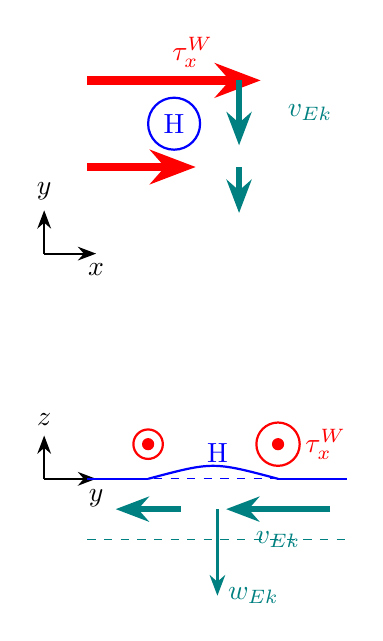
\begin{tikzpicture}[scale=1.1, >=Stealth]



    \draw[thick, red, -{Stealth[scale=1]}, line width=3pt] (0, 2) -- (2,2) node[midway, above] {$\ \ \ \ \tau_x^W$};
    \draw[thick, red, -{Stealth[scale=1]}, line width=3pt] (0, 1) -- (1.25,1);
    % teal arrow pointing down at x=1.75, y=2
    \draw[thick, teal, -{Stealth[scale=1]}, line width=2pt] (1.75,2) -- (1.75,1.25) node[midway, right] {$\ \ \ \ v_{Ek}$};
    \draw[thick, teal, -{Stealth[scale=1]}, line width=2pt] (1.75,1) -- (1.75,.469);

    \node[text=blue] at (1,1.5) {H};
    % draw a large circle around this:
    \draw[thick, blue] (1+0.3,1.5) arc[start angle=0, end angle=360, radius=0.3];



    % small axes indicating x and y directions:
    \draw[->, thick] (-0.5,0) -- (0.1,0) node[below] {$x$};
    \draw[->, thick] (-0.5,0) -- (-0.5,0.5) node[above] {$y$};

    % make another part of the figure below the part above:
    \begin{scope}[yshift=-2.6cm]
        % small axes indicating x and y directions:
        \draw[->, thick] (-0.5,0) -- (0.1,0) node[below] {$y$};
        \draw[->, thick] (-0.5,0) -- (-0.5,0.5) node[above] {$z$};

        \draw[dashed, blue] (0,0) -- (3,0.0) node[midway, above]{};
        \draw[dashed, teal] (0,-0.7) -- (3,-0.7) node[midway, above]{};


        \tikzCircleDotLabel{2.2}{0.4}{0.25}{red}{$\tau^W_x$}
        \tikzCircleDotLabel{0.7}{0.4}{0.17}{red}{}

        % draw a shallow arc, concave down between x= 2.2 and 0.7 with y =0 on the end points:
        \draw[thick, blue] (2.2,0) .. controls (0.7+0.75,0.2) .. (0.7,0);
        \node[text=blue] at (1.5,0.3) {H};

        \draw[thick, blue] (0, 0) -- (0.7, 0);
        \draw[thick, blue] (2.2, 0) -- (3, 0);
        \draw[thick, teal, -{Stealth[scale=1]}, line width=2pt] (2.8,-0.35) -- (1.6,-0.35) node {};
        % put a label below this arrow:
        \node[text=teal] at (2.2,-0.7) {$v_{Ek}$};

        \draw[thick, teal, -{Stealth[scale=1]}, line width=2pt] (.75/2 + 0.7,-0.35) -- (-.75/2 + 0.7,-0.35) node {};

        \draw[thick, teal, -{Stealth[scale=1]}, line width=1pt] (1.5 ,-0.35) -- (1.5, -1.35) node[right ]{$w_{Ek}$};


    \end{scope}

%
\end{tikzpicture}
\end{document}
